\documentclass[12pt,a4paper]{article}

% ============================================================
% FuelBot Lite - Informe académico de ejecución
% Compilar en Overleaf con pdfLaTeX.
% Las figuras deben estar en la carpeta figuras/.
% ============================================================

\usepackage[utf8]{inputenc}
\usepackage[T1]{fontenc}
\usepackage[spanish,es-noshorthands]{babel}
\usepackage{lmodern}
\usepackage[a4paper,margin=2.5cm]{geometry}
\usepackage{graphicx}
\usepackage{booktabs}
\usepackage{longtable}
\usepackage{array}
\usepackage{tabularx}
\usepackage{makecell}
\usepackage{float}
\usepackage{placeins}
\usepackage{caption}
\usepackage{subcaption}
\usepackage{xcolor}
\usepackage{amsmath}
\usepackage{enumitem}
\usepackage{fancyhdr}
\usepackage{listings}
\usepackage{upquote}
\usepackage{tikz}
\usepackage{pgfplots}
\usepackage{hyperref}
\usepackage{url}
\usepackage{microtype}

\graphicspath{{figuras/}}
\setlength{\headheight}{14pt}
\usetikzlibrary{arrows.meta,positioning,fit,backgrounds,calc}
\pgfplotsset{compat=1.18}

\definecolor{fbforest}{HTML}{26382E}
\definecolor{fbdeep}{HTML}{405A3F}
\definecolor{fbolive}{HTML}{617A50}
\definecolor{fbleaf}{HTML}{91A77B}
\definecolor{fbsage}{HTML}{D9DED5}
\definecolor{fbmineral}{HTML}{F7F8F5}
\definecolor{fbgraphite}{HTML}{26342B}
\definecolor{fbbajo}{HTML}{B4453C}
\definecolor{fbmedio}{HTML}{C58A2B}
\definecolor{fbalto}{HTML}{4E7C46}

\hypersetup{
  colorlinks=true,
  linkcolor=fbdeep,
  citecolor=fbdeep,
  urlcolor=fbolive,
  pdftitle={FuelBot Lite: informe académico de ejecución},
  pdfauthor={Proyecto FuelBot Lite}
}

\captionsetup{font=small,labelfont=bf,justification=centering}
\setlength{\parskip}{0.35em}
\setlength{\parindent}{0pt}
\renewcommand{\arraystretch}{1.15}

\pagestyle{fancy}
\fancyhf{}
\fancyhead[L]{\small FuelBot Lite}
\fancyhead[R]{\small Informe técnico-académico}
\fancyfoot[C]{\thepage}
\renewcommand{\headrulewidth}{0.4pt}

\lstdefinestyle{codigo}{
  basicstyle=\ttfamily\footnotesize,
  breaklines=true,
  breakatwhitespace=false,
  columns=fullflexible,
  keepspaces=true,
  showstringspaces=false,
  frame=single,
  rulecolor=\color{fbsage},
  backgroundcolor=\color{fbmineral},
  keywordstyle=\color{fbdeep}\bfseries,
  commentstyle=\color{fbolive},
  stringstyle=\color{fbgraphite},
  numbers=left,
  numberstyle=\tiny\color{gray},
  numbersep=8pt,
  captionpos=b,
  extendedchars=true,
  inputencoding=utf8,
  literate={á}{{\'a}}1 {é}{{\'e}}1 {í}{{\'i}}1 {ó}{{\'o}}1 {ú}{{\'u}}1
           {Á}{{\'A}}1 {É}{{\'E}}1 {Í}{{\'I}}1 {Ó}{{\'O}}1 {Ú}{{\'U}}1
           {ñ}{{\~n}}1 {Ñ}{{\~N}}1 {ü}{{\"u}}1 {¿}{{?`}}1 {¡}{{!`}}1
}
\lstset{style=codigo}

\newcommand{\fuel}{\texttt{fuel}}
\newcommand{\vista}[1]{\texttt{#1}}
\newcommand{\archivo}[1]{\texttt{#1}}

\begin{document}

% ============================================================
% PORTADA
% ============================================================
\begin{titlepage}
\centering
\vspace*{1.2cm}

{\color{fbdeep}\rule{\linewidth}{1.2pt}}\\[0.5cm]
{\Large\scshape Plataforma académica de inteligencia energética\par}
\vspace{1.0cm}

{\Huge\bfseries FuelBot Lite\par}
\vspace{0.45cm}
{\LARGE Inteligencia energética para el departamento de La Paz\par}
\vspace{0.8cm}

{\Large Informe académico de ejecución:\\[0.18cm]
extracción de datos, alojamiento en Supabase y despliegue\par}
\vspace{0.4cm}
{\color{fbdeep}\rule{\linewidth}{1.2pt}}

\vfill

\begin{tabular}{rl}
\textbf{Proyecto:} & FuelBot Lite, versión 2.0.0\\
\textbf{Fuentes:} & ANH y YPFB (datos públicos)\\
\textbf{Periodo documentado:} & 12--13 de noviembre de 2026\\
\textbf{Entorno validado:} & R 4.6.2, Windows, Supabase PostgreSQL\\
\textbf{Autor:} & [Nombre del autor]\\
\textbf{Fecha:} & 13 de noviembre de 2026\\
\end{tabular}

\vfill
{\small Documento elaborado a partir del repositorio real del proyecto.\\
No se incluyen credenciales ni valores de configuración sensibles.}
\end{titlepage}

% ============================================================
% RESUMEN
% ============================================================
\pagenumbering{roman}
\section*{Resumen}
\addcontentsline{toc}{section}{Resumen}

Este informe documenta la ejecución técnica de FuelBot Lite, una plataforma académica que integra datos públicos de la Agencia Nacional de Hidrocarburos (ANH) y de Yacimientos Petrolíferos Fiscales Bolivianos (YPFB) para analizar la situación de los combustibles en el departamento de La Paz. El trabajo cubre el ciclo completo: extracción y normalización de datos, carga idempotente en una base PostgreSQL alojada en Supabase, publicación de vistas de consulta, construcción de un tablero en R Shiny, incorporación de un agente conversacional basado en Gemini con acceso SQL de solo lectura, y verificación funcional en escritorio y móvil.

La extracción combina tres rutas: la API pública de ANH, el bloque JSON embebido en la página de consulta de YPFB y los archivos CSV históricos del repositorio \texttt{sociedatos/bo-combustible}. El pipeline en R aplica control de ritmo, reintentos, copia cruda comprimida con huella SHA-256, normalización de fechas y textos, validación de coordenadas e inserción mediante \texttt{ON CONFLICT} para evitar duplicados. La base separa los datos operativos en el esquema \fuel{} y expone vistas con semántica explícita; la aplicación y el agente usan exclusivamente el rol \texttt{agente\_ro}, sin permisos de escritura.

La instancia consultada al cierre contiene 126 estaciones, 259 pares estación-producto en la vista de saldo actual, 232 pares con saldo bajo, 5 medios y 22 altos, además de 33 despachos confirmados y 160 registros de programación de YPFB para el 13 de noviembre de 2026. El agente respondió correctamente una consulta de prueba y mostró la evidencia SQL. La aplicación se validó localmente con Chrome headless en 1440 y 390 píxeles, sin errores de JavaScript. El despliegue en la nube de la aplicación no forma parte de los artefactos actuales del repositorio; el pipeline de datos sí cuenta con un workflow de GitHub Actions. Esta distinción se explicita en el informe para no atribuir al proyecto un despliegue que no fue ejecutado.

\textbf{Palabras clave:} ETL, datos abiertos, R, Shiny, Supabase, PostgreSQL, Gemini, visualización, trazabilidad.

\newpage
\tableofcontents
\newpage
\pagenumbering{arabic}

% ============================================================
% 1. INTRODUCCIÓN
% ============================================================
\section{Introducción}

\subsection{Contexto y problema}

La disponibilidad de combustibles en Bolivia se comunica a través de fuentes públicas fragmentadas. La ANH publica saldos reportados por estación de servicio y producto; YPFB publica despachos de cisternas, programación y resumenes por distrito comercial. Cada fuente tiene una semántica distinta y una frecuencia propia. Un saldo reportado no equivale a disponibilidad física, un despacho confirmado no garantiza que el producto este disponible en una estación y una programación es un volumen planificado que puede no haber sido atendido.

Para un análisis académico, el problema no es solo visualizar datos: es construir un flujo reproducible que preserve la procedencia, distinga los tipos de dato y permita auditar cada cifra. FuelBot Lite aborda ese problema con un pipeline en R, una base PostgreSQL hospedada en Supabase y un tablero Shiny con un agente que consulta la base mediante SQL de solo lectura.

\subsection{Objetivos}

\textbf{Objetivo general.} Documentar y evaluar la ejecución de un sistema de integración, almacenamiento, visualización y consulta conversacional de datos públicos de combustibles para el departamento de La Paz.

\textbf{Objetivos específicos.}
\begin{enumerate}[leftmargin=1.2cm]
  \item Describir las fuentes de datos, los mecanismos de extracción y las reglas de limpieza aplicadas.
  \item Explicar el modelo de datos, las vistas y el esquema de seguridad implementados en Supabase.
  \item Analizar la carga idempotente, la trazabilidad de las capturas y los controles de calidad.
  \item Documentar la arquitectura del tablero Shiny y del agente Gemini.
  \item Distinguir el despliegue efectivamente validado del despliegue previsto o recomendado.
  \item Presentar los resultados de la validación con datos reales y reconocer las limitaciones.
\end{enumerate}

\subsection{Alcance y delimitaciones}

El alcance territorial es el departamento de La Paz, codificado como \texttt{DEPARTAMENTO\_ID=2} en la fuente ANH, y el distrito comercial \texttt{LPZ} en YPFB. El alcance temporal de la instancia consultada es el 13 de noviembre de 2026, aunque el pipeline admite la carga de históricos mediante los CSV del repositorio de referencia.

No se incluye la API móvil de ANH que utiliza una clave incrustada y un agente de usuario simulado; esa ruta se excluyó por criterios académicos y de uso responsable. Tampoco se implementan PostGIS, motores de búsqueda de texto completo, un crawler multipágina ni un despliegue cloud de la aplicación. Estas ausencias se declaran como límites, no como resultados.

\subsection{Estructura del documento}

La sección \ref{sec:marco} presenta el marco tecnológico. La sección \ref{sec:arquitectura} describe la arquitectura. La sección \ref{sec:fuentes} detalla la extracción. La sección \ref{sec:supabase} explica el almacenamiento y la seguridad. La sección \ref{sec:calidad} resume el procesamiento y la calidad. La sección \ref{sec:dashboard} documenta el tablero. La sección \ref{sec:agente} describe el agente. La sección \ref{sec:despliegue} distingue el despliegue real del previsto. La sección \ref{sec:validacion} presenta las pruebas y resultados. La sección \ref{sec:discusion} discute alcances y límites. Finalmente se presentan las conclusiones, las referencias y los apéndices reproducibles.

% ============================================================
% 2. MARCO
% ============================================================
\section{Marco conceptual y tecnológico}\label{sec:marco}

\subsection{Extracción, transformación y carga}

El proyecto implementa un proceso ETL (extraer, transformar y cargar) con características de \emph{idempotencia}: repetir una corrida no debe duplicar filas ni alterar el resultado esperado. La idempotencia se apoya en claves primarias estables y en la clausula \texttt{ON CONFLICT} de PostgreSQL. En un contexto académico, esta propiedad es relevante porque permite reproducir la carga, corregir errores y volver a ejecutar el pipeline sin reconstruir la base.

La transformación incluye normalización de fechas, conversión de identificadores, reparación de textos con codificación dañada, validación del recuadro geográfico de Bolivia y deduplicación. La carga conserva una copia cruda comprimida y una huella SHA-256 para auditar que el dato transformado proviene de una respuesta concreta.

\subsection{Web scraping y uso responsable}

No todas las fuentes ofrecen una API documentada. La página de YPFB entrega los datos dentro de un bloque \texttt{<script id="datos-publicos">} con JSON; el pipeline extrae ese bloque con una expresión regular, sin navegador automatizado. La ANH ofrece un endpoint JSON. En ambos casos se usa un agente de usuario identificable, un limite de ritmo, tiempo de espera y reintentos. No se falsifica la identidad del cliente ni se intenta evadir bloqueos.

\subsection{Alojamiento en Supabase}

Supabase proporciona PostgreSQL administrado, editor SQL y un pooler de conexiones. El proyecto crea un esquema propio, \fuel{}, para no exponer las tablas por la API REST automática de Supabase y para separar el modelo operativo de las vistas de consulta. La aplicación se conecta con SSL obligatorio y con un usuario de solo lectura.

\subsection{Visualización y agentes}

R Shiny organiza la interfaz en modulos y actualiza los datos mediante \texttt{reactivePoll}. bslib aporta el tema Bootstrap 5; Leaflet renderiza el mapa; Plotly construye los gráficos; DT presenta las tablas. El agente utiliza \emph{function calling} de Gemini: el modelo no recibe acceso directo a la base, sino una herramienta \texttt{ejecutar\_sql} que valida la consulta y la ejecuta con el rol de lectura. La aplicación muestra la consulta como evidencia.

\begin{table}[H]
\centering
\small
\caption{Componentes tecnológicos y función en el proyecto.}
\label{tab:componentes}
\begin{tabularx}{\linewidth}{@{}l X@{}}
\toprule
\textbf{Componente} & \textbf{Función} \\
\midrule
R 4.6.2 & Lenguaje único del pipeline, el tablero y el agente. \\
httr2, jsonlite & Solicitudes HTTP, reintentos y lectura de JSON. \\
dplyr, purrr, stringr & Transformación, iteración y limpieza de textos. \\
readr & Lectura de los CSV históricos como texto. \\
digest & Huellas SHA-256 de los crudos y claves MD5 de YPFB. \\
DBI, RPostgres & Conexión a PostgreSQL y ejecución de SQL. \\
Supabase & PostgreSQL administrado, editor SQL y pooler. \\
Shiny, bslib & Interfaz reactiva y tema visual. \\
Leaflet, Plotly, DT & Mapa, gráficos y tablas interactivas. \\
Gemini API & Modelo de lenguaje con function calling. \\
GitHub Actions & Automatización programada del pipeline. \\
\bottomrule
\end{tabularx}
\end{table}

% ============================================================
% 3. ARQUITECTURA
% ============================================================
\section{Arquitectura del sistema}\label{sec:arquitectura}

La arquitectura se organiza en cinco capas: fuentes, extracción y transformación, almacenamiento, presentación e inteligencia. La figura \ref{fig:arquitectura} resume el flujo.

\begin{figure}[H]
\centering
\resizebox{0.98\linewidth}{!}{%
\begin{tikzpicture}[
  font=\small,
  >=Latex,
  src/.style={draw=fbdeep, fill=fbmineral, rounded corners=4pt,
              align=center, minimum width=3.1cm, minimum height=1.15cm},
  proc/.style={draw=fbolive, fill=fbsage!45, rounded corners=4pt,
               align=center, minimum width=3.4cm, minimum height=1.3cm},
  store/.style={draw=fbforest, fill=fbforest!8, rounded corners=4pt,
                align=center, minimum width=3.5cm, minimum height=1.5cm},
  app/.style={draw=fbdeep, fill=white, rounded corners=4pt,
              align=center, minimum width=3.4cm, minimum height=1.35cm},
  ops/.style={draw=fbmedio, fill=fbmedio!10, rounded corners=4pt,
              align=center, minimum width=3.4cm, minimum height=1.0cm},
  arrow/.style={->, thick, draw=fbdeep}
]

\node[src] (anh) at (0,2.1) {ANH\\API JSON};
\node[src] (ypfb) at (0,0) {YPFB\\HTML + JSON};
\node[src] (repo) at (0,-2.1) {Repo\\CSV históricos};

\node[proc] (etl) at (4.7,0) {Pipeline R\\extraer -- limpiar -- cargar};
\node[ops] (gha) at (4.7,-2.7) {GitHub Actions\\cron cada 2 h};

\node[store] (db) at (9.2,0) {Supabase\\PostgreSQL\\esquema \fuel{}};
\node[store] (vistas) at (9.2,-2.7) {Vistas \vista{v\_*}\\rol \texttt{agente\_ro}};

\node[app] (shiny) at (13.5,1.1) {Dashboard\\Shiny};
\node[app] (gem) at (13.5,-1.1) {Agente\\Gemini};

\draw[arrow] (anh) -- (etl);
\draw[arrow] (ypfb) -- (etl);
\draw[arrow] (repo) -- (etl);
\draw[arrow] (gha) -- (etl);
\draw[arrow] (etl) -- node[above,font=\scriptsize]{ON CONFLICT} (db);
\draw[arrow] (db) -- (vistas);
\draw[arrow] (vistas) -- (shiny);
\draw[arrow] (vistas) -- (gem);
\draw[arrow] (gem) -- node[right,font=\scriptsize]{SQL de lectura} (shiny);

\node[draw=gray!45, dashed, rounded corners=6pt, fit=(etl)(gha), inner sep=12pt,
      label={[font=\scriptsize,text=gray]above:Capa de extracción y carga}] {};
\node[draw=gray!45, dashed, rounded corners=6pt, fit=(db)(vistas), inner sep=12pt,
      label={[font=\scriptsize,text=gray]above:Capa de datos}] {};
\node[draw=gray!45, dashed, rounded corners=6pt, fit=(shiny)(gem), inner sep=12pt,
      label={[font=\scriptsize,text=gray]above:Capa de consumo}] {};

\end{tikzpicture}%
}
\caption{Arquitectura general de FuelBot Lite. El agente y el tablero consumen exclusivamente las vistas del esquema \fuel{} mediante el rol de lectura.}
\label{fig:arquitectura}
\end{figure}

\subsection{Flujo de datos}

\begin{enumerate}[leftmargin=1.2cm]
  \item El pipeline solicita los datos a ANH, a YPFB o a los CSV históricos.
  \item Guarda una copia cruda comprimida y calcula su SHA-256.
  \item Normaliza los registros y los carga en las tablas del esquema \fuel{}.
  \item Registra la corrida en \vista{ingesta\_log}.
  \item Las vistas traducen el modelo operativo a un modelo de consulta con nombres y semántica estables.
  \item El tablero y el agente consultan las vistas con el rol \texttt{agente\_ro}.
\end{enumerate}

\subsection{Decisiones de arquitectura}

\begin{itemize}[leftmargin=1.2cm]
  \item \textbf{Un solo lenguaje:} R reduce la fricción entre extracción, análisis, visualización y agente.
  \item \textbf{Base administrada:} Supabase evita operar un servidor PostgreSQL y un contenedor propio.
  \item \textbf{Esquema propio:} \fuel{} separa los datos del proyecto y no queda expuesto automáticamente por la API REST.
  \item \textbf{Vistas como contrato:} el tablero y el agente dependen de vistas, no de tablas; se evita acoplar la interfaz al modelo de carga.
  \item \textbf{Dos identidades:} escritura solo para el pipeline; lectura para la aplicación y el agente.
  \item \textbf{Trazabilidad:} crudos con hash, fechas de captura, fecha de reporte y bitacora de ingesta.
\end{itemize}

% ============================================================
% 4. FUENTES Y EXTRACCIÓN
% ============================================================
\section{Fuentes de datos y extracción}\label{sec:fuentes}

\subsection{ANH: saldos por estación y producto}

La ANH se consulta mediante el endpoint público \url{https://abastecimiento.prod.anh.gob.bo/api/estaciones}. El pipeline recorre los cuatro productos configurados y envía los parámetros \texttt{departamento=2} y \texttt{producto=0..3}. La respuesta se interpreta como JSON y se valida que el mensaje sea \texttt{OK}, que \texttt{oResultado} sea una lista y que contenga registros.

Los campos de interes son la estación, el producto, el saldo en litros, el estado reportado, la fecha de actualización del sistema, la fecha de última venta, el despacho en curso y las coordenadas. La Tabla \ref{tab:anh-campos} resume el tratamiento.

\begin{table}[H]
\centering
\small
\caption{Tratamiento de los campos de ANH.}
\label{tab:anh-campos}
\begin{tabularx}{\linewidth}{@{}l X@{}}
\toprule
\textbf{Campo} & \textbf{Tratamiento} \\
\midrule
\texttt{id\_eess} & Conversión a entero y luego a texto; se descarta si falta. \\
\texttt{id\_producto} & Conversión a entero; se usa para el nombre del producto. \\
\texttt{fecha\_actualizacion} & Se reemplaza por la hora de captura del pipeline. \\
\texttt{fecha\_actualizacion\_sistema} & Normalización a \texttt{YYYY-MM-DD HH:MM:SS}. \\
\texttt{saldo\_litros} & Se conserva como numérico; puede ser nulo. \\
\texttt{saldo\_estado} & Minusculas y espacios recortados; se esperan bajo, medio o alto. \\
\texttt{nombre, direccion, zona} & Reparación de mojibake y conservación del texto. \\
\texttt{lat, lng} & Conversión numérica y validación del recuadro de Bolivia. \\
\texttt{departamento\_id} & Filtro estricto al departamento configurado. \\
\bottomrule
\end{tabularx}
\end{table}

La normalización se implementa en \archivo{pipeline/01\_extraer\_anh.R}. Entre sus reglas se encuentran:
\begin{itemize}[leftmargin=1.2cm]
  \item descartar filas sin estación, producto o fecha de captura;
  \item descartar filas de otro departamento;
  \item advertir si aparece un estado distinto de bajo, medio o alto;
  \item anular coordenadas fuera del recuadro aproximado de Bolivia;
  \item conservar una sola fila por combinación fecha-estación-producto, con la última aparición;
  \item conservar para la tabla de estaciones el registro más reciente de cada estación.
\end{itemize}

El resultado se separa en dos conjuntos: \texttt{saldos} y \texttt{estaciones}. Ambos se cargan en Supabase. La respuesta cruda de los cuatro productos se guarda como JSON comprimido en \texttt{data/raw/anh/}.

\subsection{YPFB: despachos, programación y resumen}

La página \url{https://consulta.ypfb.gob.bo/} contiene un bloque de datos embebido:

\begin{lstlisting}[language=HTML,caption={Estructura del bloque de datos de YPFB (extracto).}]
<script type="application/json" id="datos-publicos">
  { "fecha_datos": "...", "distritos": [...], "datos": {...} }
</script>
\end{lstlisting}

El extractor localiza el bloque con una expresión regular, lo parsea con \texttt{jsonlite} y recorre la estructura \texttt{datos} por distrito y producto. Solo conserva el distrito configurado (\texttt{LPZ}). De cada combinación extrae tres conjuntos:
\begin{description}[leftmargin=1.2cm]
  \item[Despachos:] cisternas, placa, estación, cliente, producto despachado, cantidad, fecha programada, fecha efectiva y condición de confirmación.
  \item[Programación:] volumen planificado, cliente, producto, canal y estado de atención.
  \item[Resumen:] litros programados, despachados y pendientes de confirmación por distrito y producto general.
\end{description}

Para evitar que dos filas legitimamente idénticas se colapsen, se construye una clave MD5 con los campos relevantes y un sufijo de repetición. La clave se usa como llave primaria en la base. La página completa se guarda como HTML comprimido en \texttt{data/raw/ypfb/}.

\subsection{Backfill histórico}

El repositorio público \texttt{sociedatos/bo-combustible} publica CSV semanales. El pipeline puede descargarlos mediante la API de contenidos de GitHub o leerlos desde un clon local. Se usan las carpetas \path{data_abastecimiento} y \path{data_ypfb/despachos}, \path{data_ypfb/programacion} y \path{data_ypfb/resumen}. Todos los campos se leen como texto y luego pasan por los mismos normalizadores que la captura en vivo.

El modo \texttt{backfill} sirve para poblar la base al inicio y como respaldo si un portal cambia o bloquea la extracción. En la instancia documentada, la base consultada contiene solo las capturas del 13 de noviembre; la capacidad de backfill existe, pero no se verificó una carga histórica completa en esta instancia.

\subsection{HTTP responsable y procedencia}

La función \texttt{pedir()} de \archivo{pipeline/00\_config.R} aplica un agente de usuario identificable, tiempo de espera de 60 segundos, un limite de 20 solicitudes por minuto y hasta tres reintentos con retroceso exponencial. La Tabla \ref{tab:http} resume las decisiones.

\begin{table}[H]
\centering
\small
\caption{Controles de extracción y trazabilidad.}
\label{tab:http}
\begin{tabularx}{\linewidth}{@{}l X@{}}
\toprule
\textbf{Control} & \textbf{Implementación} \\
\midrule
Identificación & \texttt{USER\_AGENT} configurable, con contacto editable. \\
Ritmo & \texttt{req\_throttle(rate = 20/60)}. \\
Espera & \texttt{req\_timeout(60)}. \\
Reintentos & Tres intentos con espera \(2^i\) segundos. \\
Crudo & JSON o HTML comprimido en \texttt{data/raw/}. \\
Integridad & SHA-256 con \texttt{digest::digest()}. \\
Bitacora & Tabla \fuel.ingesta\_log con inicio, fin, filas, estado y mensaje. \\
\bottomrule
\end{tabularx}
\end{table}

El SHA-256 no se usa como identificador de negocio; sirve para verificar que el archivo crudo conservado corresponde a la respuesta que origino una carga.

% ============================================================
% 5. SUPABASE
% ============================================================
\section{Almacenamiento en Supabase}\label{sec:supabase}

\subsection{Aprovisionamiento}

El proyecto se creó en Supabase y se configuró la conexión mediante el \emph{Session pooler}, que facilita el acceso desde redes IPv4. La cadena de conexión se guarda en \texttt{.Renviron} y no se versiona. La conexión utiliza \texttt{sslmode=require}. El esquema y las vistas se ejecutan manualmente desde el editor SQL de Supabase, en el orden \archivo{sql/01\_esquema.sql} y \archivo{sql/02\_vistas\_y\_rol.sql}.

\subsection{Modelo de tablas}

\begin{table}[H]
\centering
\small
\caption{Tablas del esquema \fuel{}.}
\label{tab:tablas}
\begin{tabularx}{\linewidth}{@{}l l X@{}}
\toprule
\textbf{Tabla} & \textbf{Clave primaria} & \textbf{Proposito} \\
\midrule
\texttt{estaciones} & \texttt{id\_eess} & Catalogo de estaciones, dirección, zona, coordenadas y departamento. \\
\texttt{saldos} & fecha, estación, producto & Una fila por captura, estación y producto; conserva el histórico. \\
\texttt{ypfb\_despachos} & \texttt{clave} & Cisternas despachadas y confirmadas. \\
\texttt{ypfb\_programacion} & \texttt{clave} & Volumen planificado y estado de atención. \\
\texttt{ypfb\_resumen} & fecha, distrito, producto & Agregado por distrito y producto general. \\
\texttt{ingesta\_log} & identidad & Bitacora de cada corrida y su resultado. \\
\bottomrule
\end{tabularx}
\end{table}

La tabla \texttt{saldos} tiene una clave foranea a \texttt{estaciones}. Se define un índice por estación, producto y fecha descendente para acelerar la vista de saldo actual. Las tablas de YPFB tienen índices por fecha de datos o fecha de despacho. El esquema se crea con \texttt{create schema if not exists} y las tablas con \texttt{create table if not exists}, de modo que el script es repetible.

\subsection{Vistas de consulta}

Las vistas son el contrato entre los datos y la aplicación. La Tabla \ref{tab:vistas} las resume.

\begin{table}[H]
\centering
\small
\caption{Vistas del esquema \fuel{} y su semántica.}
\label{tab:vistas}
\begin{tabularx}{\linewidth}{@{}l X@{}}
\toprule
\textbf{Vista} & \textbf{Contenido} \\
\midrule
\vista{v\_productos} & Mapa de los cuatro identificadores a nombres de producto. \\
\vista{v\_estaciones} & Catalogo con una ciudad aproximada derivada del prefijo de la dirección. \\
\vista{v\_saldo\_actual} & Último registro por estación y producto, con antigüedad en horas y \texttt{tipo\_dato}. \\
\vista{v\_saldo\_historico} & Serie completa de saldos; debe consultarse con filtros de fecha y limite. \\
\vista{v\_ypfb\_despachos} & Despachos con el alias \texttt{litros\_despachados}. \\
\vista{v\_ypfb\_programacion} & Programación con el alias \texttt{litros\_programados}. \\
\vista{v\_ypfb\_resumen} & Resumen por distrito y producto. \\
\vista{v\_fuentes} & Fuente, descripción, URL y última ingesta exitosa. \\
\vista{v\_cobertura} & Rango temporal y cantidad de filas por conjunto. \\
\bottomrule
\end{tabularx}
\end{table}

La vista \vista{v\_saldo\_actual} usa \texttt{distinct on (id\_eess, id\_producto)} y ordena por fecha de captura descendente. La antigüedad se calcula respecto de la hora de Bolivia. Cada vista de datos incorpora una columna \texttt{tipo\_dato} para impedir que el consumidor confunda saldo reportado, despacho confirmado o programación.

\subsection{Carga idempotente}

La carga sigue tres pasos: se escribe el lote en una tabla temporal con todas las columnas como texto, se ejecuta un \texttt{INSERT ... SELECT} que convierte los tipos y aplica \texttt{nullif}, y se resuelve el conflicto con \texttt{ON CONFLICT}. Los lotes son de hasta 20\,000 filas y cada lote se ejecuta dentro de una transacción.

\begin{lstlisting}[language=SQL,caption={Estrategia de carga idempotente (extracto).}]
insert into fuel.saldos (fecha_actualizacion, id_eess, id_producto, ...)
select nullif("fecha_actualizacion", '')::timestamp,
       nullif("id_eess", '')::numeric::integer,
       nullif("id_producto", '')::numeric::smallint,
       ...
from tmp_saldos
on conflict (fecha_actualizacion, id_eess, id_producto) do nothing;
\end{lstlisting}

Las estaciones se actualizan con los datos más recientes. En programación se actualizan la fecha de captura, el estado de atención y el volumen. Los despachos y los saldos no se sobrescriben: una nueva captura es una fila nueva. La bitacora se registra incluso cuando la corrida falla, con estado \texttt{error} y el mensaje correspondiente.

\subsection{Seguridad y mínimo privilegio}

El esquema aplica \texttt{revoke all on all tables in schema fuel from public}. El rol \texttt{agente\_ro} se crea con \texttt{nosuperuser}, \texttt{nocreatedb}, \texttt{nocreaterole} y \texttt{noinherit}. Además:
\begin{itemize}[leftmargin=1.2cm]
  \item se establece \texttt{default\_transaction\_read\_only = on};
  \item se fija un \texttt{statement\_timeout} de 8 segundos;
  \item se define \texttt{search\_path = fuel};
  \item se revocan todos los permisos sobre tablas;
  \item se concede \texttt{select} solo sobre las nueve vistas.
\end{itemize}

Durante la validación se comprobó que el rol es \texttt{agente\_ro} y que la transacción es de solo lectura. Un intento de consultar directamente \fuel.estaciones devuelve \emph{permission denied}; este comportamiento es evidencia de que el mínimo privilegio funciona, no un defecto.

\textbf{Riesgo detectado.} El archivo \archivo{sql/02\_vistas\_y\_rol.sql} contiene una contraseña escrita en el repositorio. En este informe no se reproduce. Se recomienda rotarla, eliminarla del historial y parametrizar su creación fuera del SQL. No se modificó el esquema durante el rediseño por la restricción de no alterar la lógica de seguridad ni el modelo de datos.

\subsection{Cobertura observada}

La vista \vista{v\_cobertura} de la instancia consultada reporta:

\begin{table}[H]
\centering
\small
\caption{Cobertura de la instancia consultada.}
\label{tab:cobertura}
\begin{tabular}{@{}lrr@{}}
\toprule
\textbf{Conjunto} & \textbf{Desde} & \textbf{Hasta} \\
\midrule
Saldos & 2026-11-13 10:29:25 & 2026-11-13 11:30:04 \\
Despachos YPFB & 2026-11-13 00:00:00 & 2026-11-13 00:00:00 \\
Programación YPFB & 2026-11-13 00:00:00 & 2026-11-13 00:00:00 \\
\bottomrule
\end{tabular}
\end{table}

La instancia contiene 518 filas de saldos, 33 despachos y 160 registros de programación. La vista de saldo actual contiene 259 pares estación-producto. La diferencia entre 518 y 259 se explica por la existencia de dos capturas del mismo día. No se debe interpretar 518 como cantidad de estaciones.

% ============================================================
% 6. CALIDAD
% ============================================================
\section{Procesamiento y calidad de datos}\label{sec:calidad}

\subsection{Reglas aplicadas}

\begin{table}[H]
\centering
\small
\caption{Reglas de calidad y su efecto.}
\label{tab:calidad}
\begin{tabularx}{\linewidth}{@{}l X@{}}
\toprule
\textbf{Regla} & \textbf{Efecto} \\
\midrule
Fechas validas & Se descartan filas sin fecha de captura o con formato no reconocido. \\
Identificadores & Se descartan filas sin estación o producto. \\
Departamento & Solo se conserva el departamento configurado. \\
Estados & Se normaliza el texto y se advierte un valor inesperado. \\
Coordenadas & Se anulan las que caen fuera del recuadro de Bolivia. \\
Duplicados ANH & Se conserva la última fila por fecha, estación y producto. \\
Duplicados YPFB & Clave MD5 más sufijo de repetición para preservar filas legitimas. \\
Mojibake & Se intenta reparar la doble codificación de textos. \\
\bottomrule
\end{tabularx}
\end{table}

\subsection{Fechas y zonas horarias}

ANH y YPFB usan marcas de tiempo con tratamientos distintos. El esquema almacena la captura y el reporte de ANH como \texttt{timestamp} sin zona, en hora de Bolivia. La fecha efectiva de despacho de YPFB se conserva como fecha y la marca horaria como \texttt{timestamptz}. La aplicación muestra la captura ANH como hora local y la ingesta como diferencia relativa para evitar mezclar zonas.

\subsection{Limitaciones semánticas}

\begin{itemize}[leftmargin=1.2cm]
  \item \textbf{Saldo reportado:} es el inventario declarado por la estación. No prueba que el combustible este disponible para la venta.
  \item \textbf{Despacho confirmado:} es una cisterna que salió de planta. No prueba que el producto haya llegado a una estación ni que este a la venta.
  \item \textbf{Programación:} es un volumen planificado; puede no haber sido atendido.
  \item \textbf{Estados:} bajo, medio y alto son categorías reportadas por ANH; los umbrales no se conocen en la fuente.
  \item \textbf{Ciudad aproximada:} se deriva del texto de la dirección y puede ser nula o incorrecta.
\end{itemize}

Estas distinciones se reflejan en la interfaz y en el system prompt del agente. No se suman programación y despacho, ni se afirma disponibilidad física a partir de un saldo.

% ============================================================
% 7. DASHBOARD
% ============================================================
\section{Tablero Shiny}\label{sec:dashboard}

\subsection{Organización}

El tablero se organiza en cuatro pestañas: Resumen, Mapa, YPFB y Agente IA. La interfaz se separo en modulos para reducir el acoplamiento:

\begin{table}[H]
\centering
\small
\caption{Modulos de la aplicación.}
\label{tab:modulos}
\begin{tabularx}{\linewidth}{@{}l X@{}}
\toprule
\textbf{Archivo} & \textbf{Responsabilidad} \\
\midrule
\archivo{app.R} & Tema, navegación, hero, footer, reactivos y registro de modulos. \\
\archivo{R/theme.R} & Paleta, tema bslib y carga de Manrope. \\
\archivo{R/components.R} & Iconos, KPI, chips, tarjetas, popups, hero y footer. \\
\archivo{R/data.R} & Función \texttt{consultar()} con reconexión y conexión de lectura. \\
\archivo{R/mod\_resumen.R} & KPIs y dos gráficos Plotly. \\
\archivo{R/mod\_mapa.R} & Filtros, estadísticas, Leaflet y tabla DT. \\
\archivo{R/mod\_ypfb.R} & KPIs, filtro por producto y tabla de programación. \\
\archivo{R/mod\_agente.R} & Chat, cuota, estados y evidencia SQL. \\
\archivo{www/motion.css} & Sistema visual y responsividad. \\
\archivo{www/custom.js} & Autoscroll, Ctrl+Enter y estado de escritura. \\
\bottomrule
\end{tabularx}
\end{table}

\subsection{Reactividad y datos}

El servidor mantiene un \texttt{reactivePoll} de 60 segundos que consulta el máximo de \texttt{fecha\_captura} y el conteo de la vista de saldo actual. Cuando cambia el valor, se invalidan los reactivos de saldos, despachos y fuentes. La aplicación no escribe en la base.

\begin{lstlisting}[language=R,caption={Latido de actualizacion de la aplicacion.}]
latido <- reactivePoll(60000, session,
  checkFunc = function() {
    r <- consultar("select max(fecha_captura)::text m, count(*) n
                    from fuel.v_saldo_actual")
    if (is.null(r)) "" else paste(r$m, r$n)
  },
  valueFunc = function() Sys.time()
)
\end{lstlisting}

\subsection{Resumen}

La pestaña Resumen presenta cuatro KPIs: estaciones con datos, última captura ANH, porcentaje de pares con saldo bajo y litros despachados por YPFB el último día. Cada KPI incluye una nota de alcance. Los gráficos son:
\begin{itemize}[leftmargin=1.2cm]
  \item barras horizontales apiladas por producto y estado de saldo;
  \item barras verticales apiladas de litros despachados por día y producto, con selector de 7, 14 o 30 días.
\end{itemize}

El eje de fechas se configura como fecha real con marcas personalizadas para evitar etiquetas duplicadas. Los miles se muestran con punto y los decimales con coma, de acuerdo con la convención local.

\subsection{Mapa y tablas}

El mapa usa teselas de OpenStreetMap, escala y marcadores circulares cuyo color representa el estado reportado. El popup muestra nombre, dirección, producto, saldo, fecha de reporte y antigüedad. La tabla inferior se sincroniza con los filtros de producto y estado. El mapa se encuadra con límites numéricos calculados a partir de los datos; el botón de centrado restablece la vista.

La tabla de YPFB muestra la programación pendiente del último día con filtro por producto. El filtro utiliza un valor centinela para permitir volver a \emph{todos los productos}, porque Selectize no representa de forma fiable una opción de valor vacío.

\subsection{Diseño y accesibilidad}

La identidad visual usa Forest Green, Deep Olive, Olive Green, Leaf Green, Sage, Metallic Grey, Mineral White y Graphite. Los tokens viven en variables CSS y en \archivo{R/theme.R}. La tipografía principal es Manrope, con respaldo en Inter y fuentes del sistema. Los estados se muestran con texto y color, el foco es visible y se respeta \texttt{prefers-reduced-motion}. En móvil se ocultan columnas secundarias para evitar el desplazamiento horizontal.

\begin{figure}[H]
\centering

\includegraphics[width=0.94\linewidth,height=0.72\textheight,keepaspectratio]{resumen.png}
\caption{Pestaña Resumen con datos reales del 13 de noviembre de 2026.}
\label{fig:resumen}
\end{figure}

\begin{figure}[H]
\centering
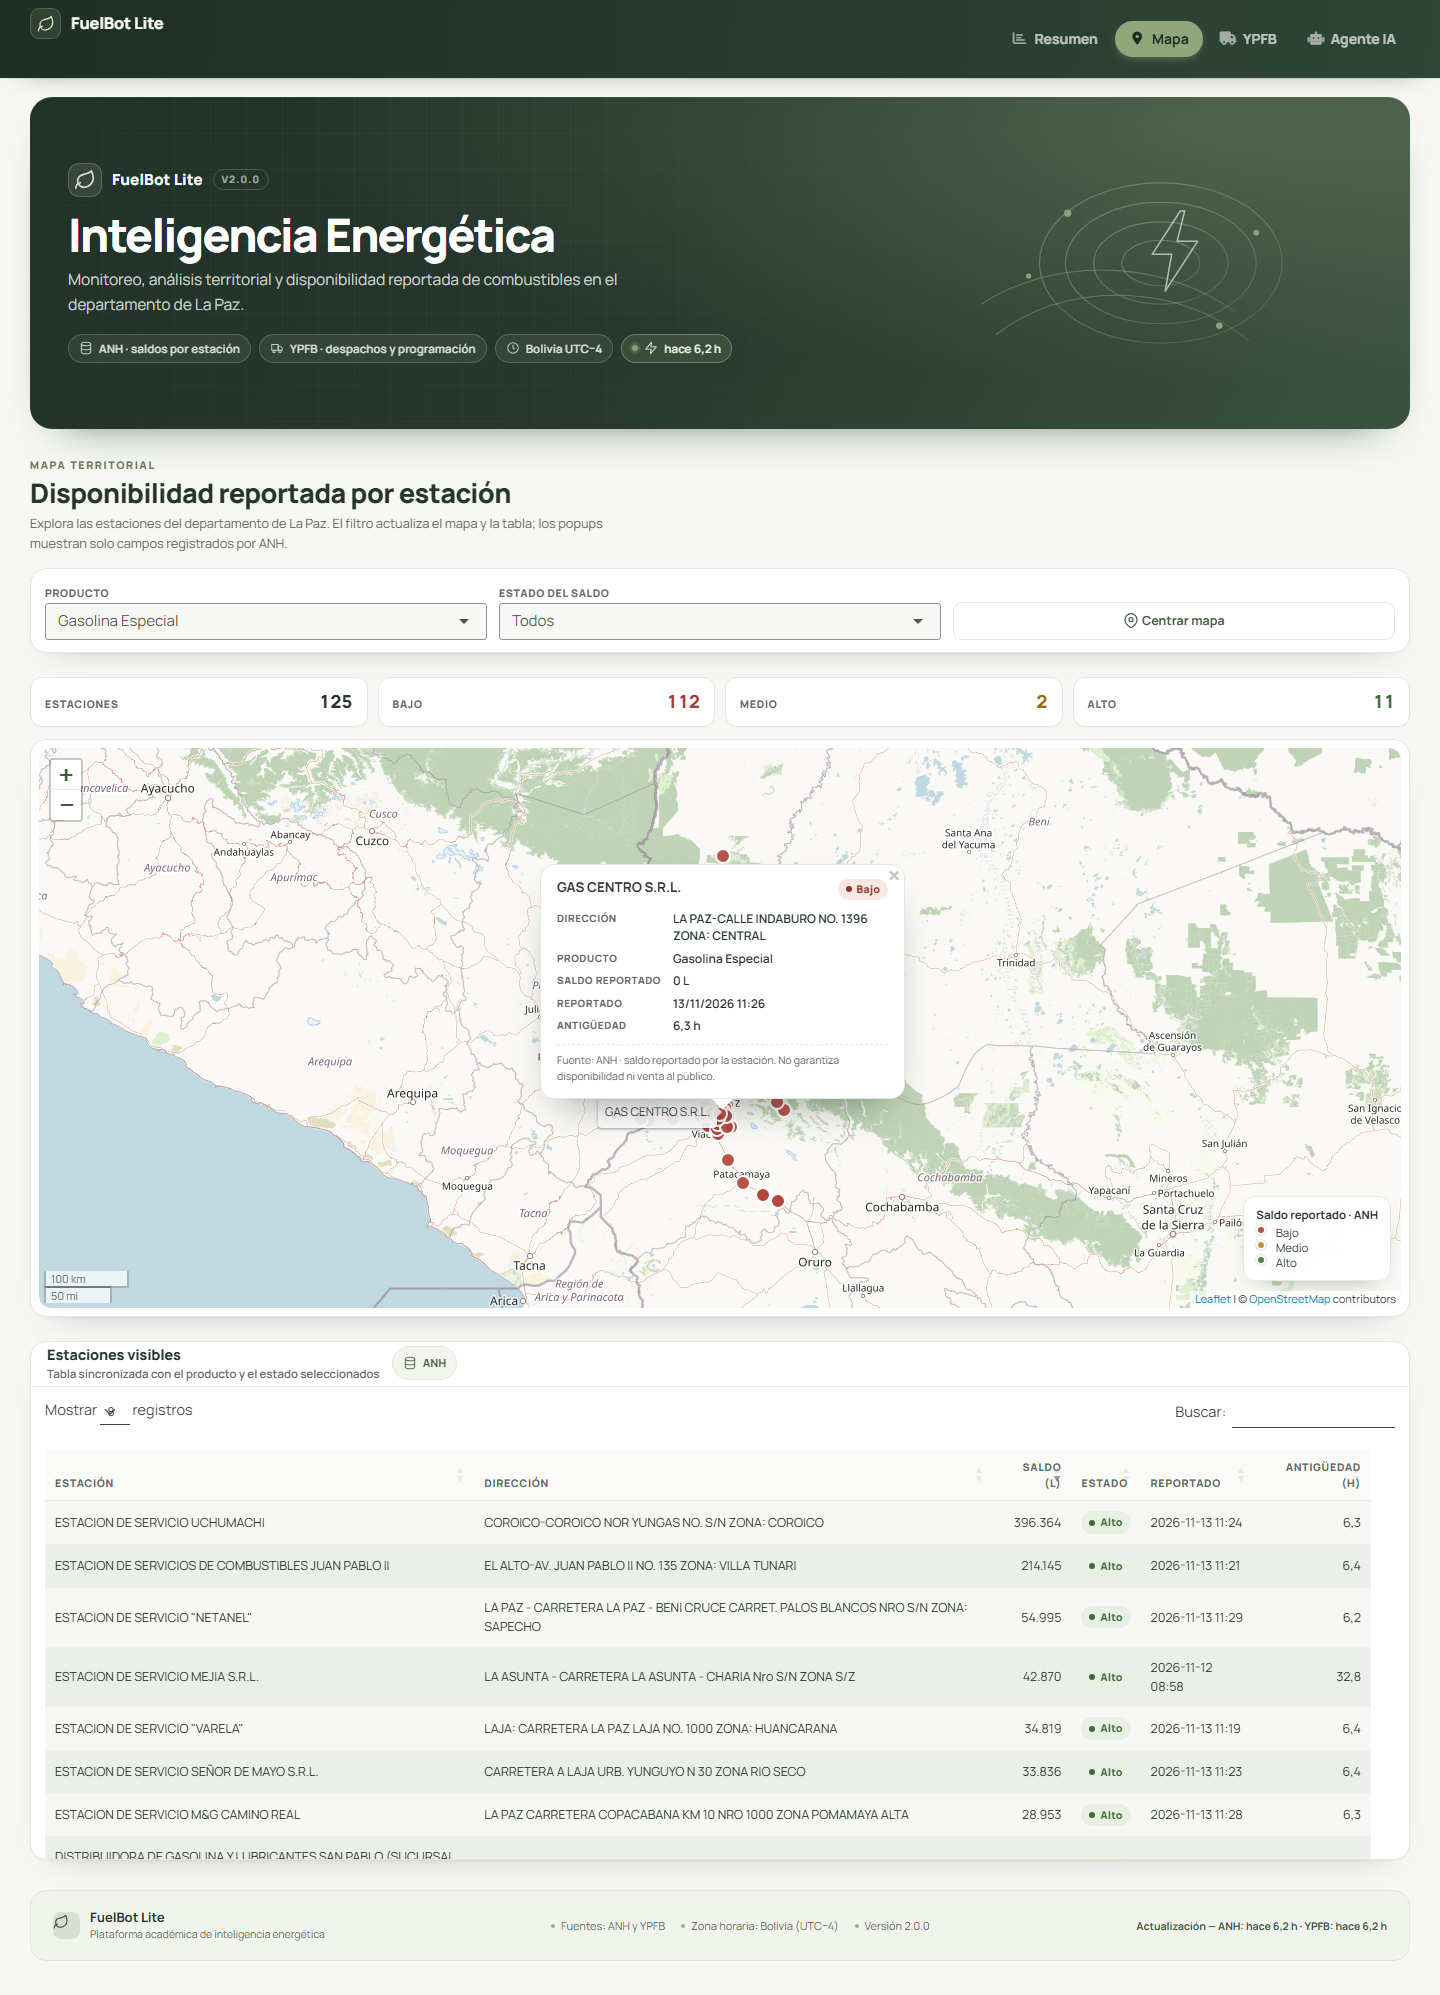
\includegraphics[width=0.94\linewidth,height=0.72\textheight,keepaspectratio]{mapa.png}
\caption{Mapa territorial con un popup de estación y la tabla sincronizada.}
\label{fig:mapa}
\end{figure}

\begin{figure}[H]
\centering
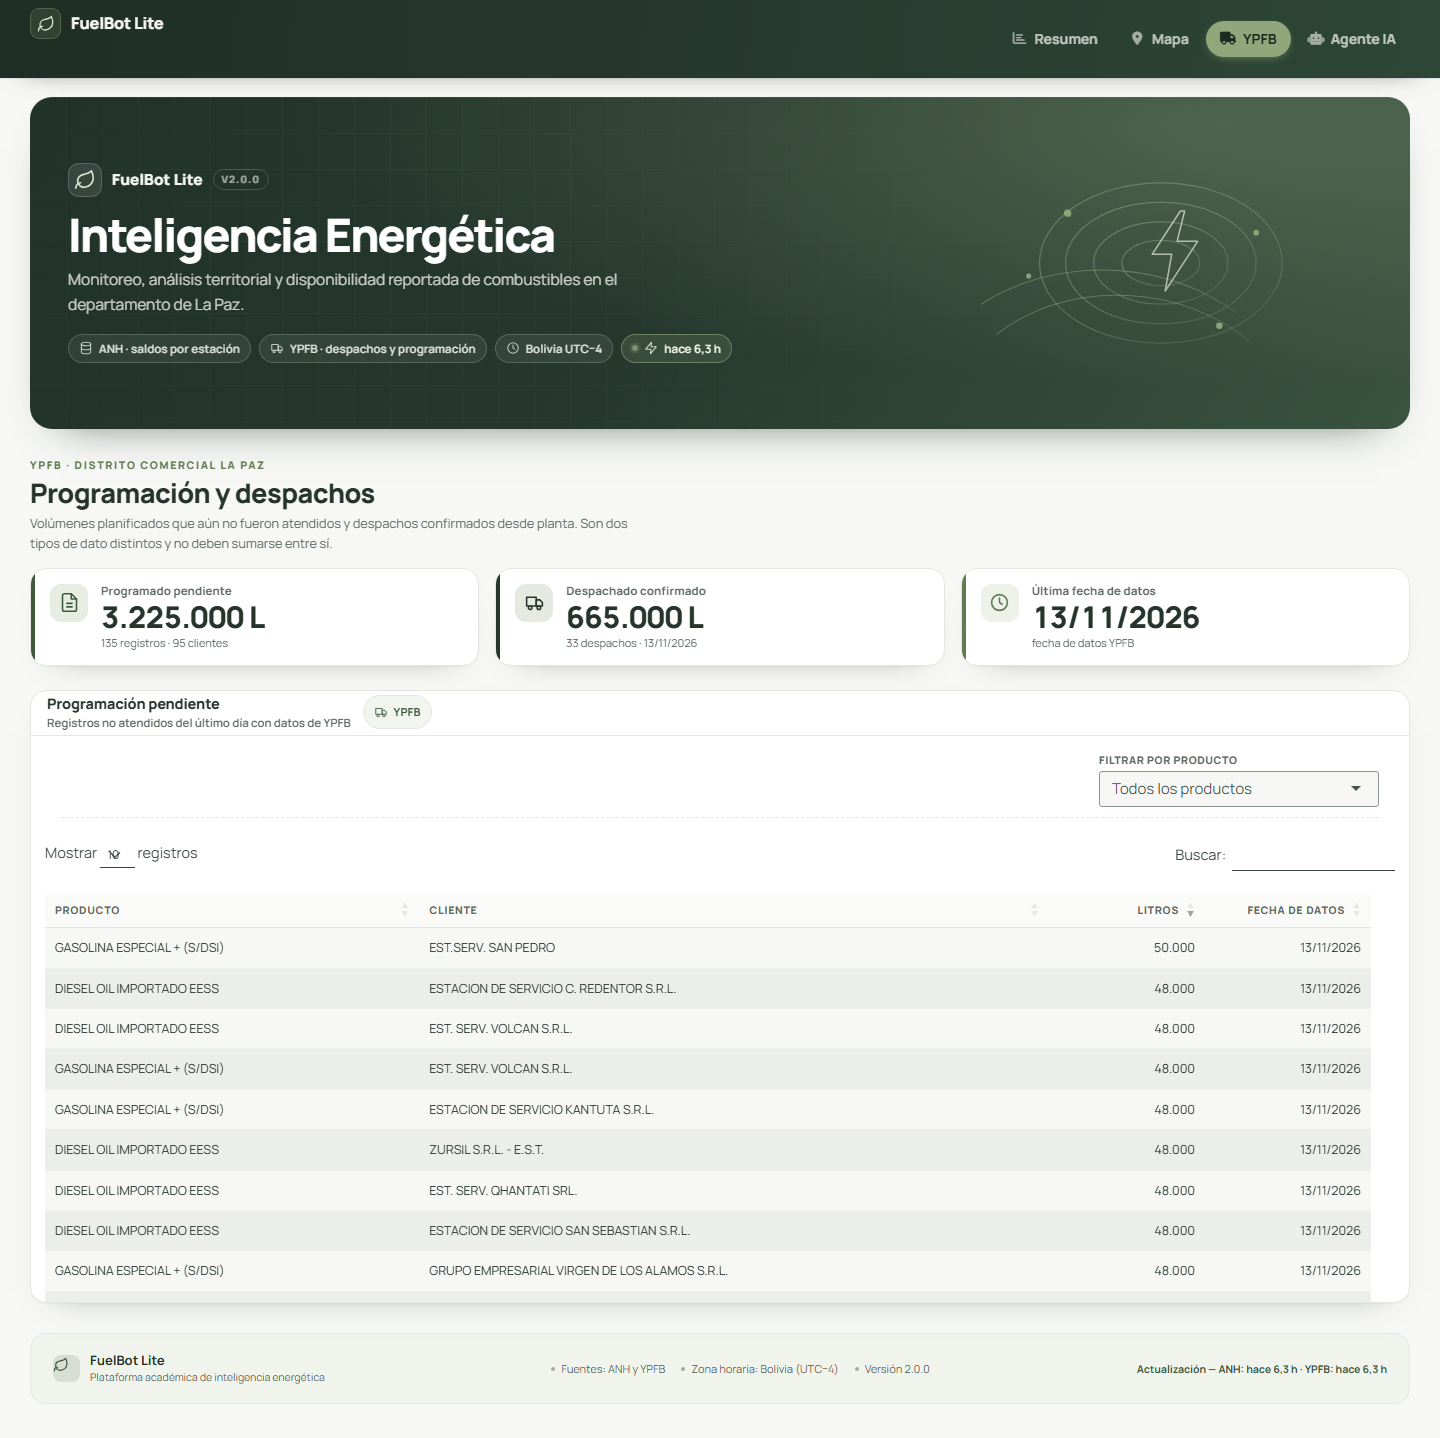
\includegraphics[width=0.94\linewidth,height=0.72\textheight,keepaspectratio]{ypfb.png}
\caption{Modulo YPFB: programación pendiente, despacho confirmado y tabla filtrable.}
\label{fig:ypfb}
\end{figure}

% ============================================================
% 8. AGENTE
% ============================================================
\section{Agente Gemini}\label{sec:agente}

\subsection{Diseño}

El agente recibe la pregunta, consulta el modelo y, si el modelo solicita una herramienta, ejecuta \texttt{ejecutar\_sql}. El ciclo se repite hasta obtener una respuesta textual o alcanzar el máximo de seis pasos. La herramienta devuelve columnas y hasta 50 filas. La aplicación muestra cada consulta en un bloque desplegable.

\begin{figure}[H]
\centering

\includegraphics[width=0.94\linewidth,height=0.68\textheight,keepaspectratio]{agente_respuesta.png}
\caption{Respuesta del agente con evidencia SQL desplegable y cuota de sesión.}
\label{fig:agente}
\end{figure}

\subsection{Defensa en profundidad}

La seguridad no depende de una sola barrera:
\begin{enumerate}[leftmargin=1.2cm]
  \item \textbf{Guardia SQL:} \texttt{validar\_sql()} acepta solo \texttt{SELECT} o \texttt{WITH}, una sola sentencia y rechaza palabras clave de escritura, funciones del sistema y comentarios.
  \item \textbf{Rol de base:} \texttt{agente\_ro} solo puede leer vistas, tiene transacción de solo lectura y un timeout de 8 segundos.
  \item \textbf{Límites:} 50 filas por consulta y 6 pasos por pregunta.
  \item \textbf{Cuota:} 3 preguntas por minuto y 30 por sesión.
  \item \textbf{Instrucciones:} el system prompt obliga a citar fuente, fecha de reporte y fecha de captura, y a no afirmar disponibilidad física.
\end{enumerate}

\begin{lstlisting}[language=R,caption={Guardia de solo lectura (extracto).}]
validar_sql <- function(consulta) {
  sql <- trimws(sub(";+\\s*$", "", trimws(consulta %||% "")))
  if (!grepl("^(select|with)\\b", sql, ignore.case = TRUE, perl = TRUE))
    return(list(error = "Solo se permiten consultas SELECT."))
  if (grepl(";", sql, fixed = TRUE))
    return(list(error = "Solo se permite una consulta por vez."))
  if (grepl(PROHIBIDAS, sql, ignore.case = TRUE, perl = TRUE))
    return(list(error = "La consulta contiene una instruccion no permitida."))
  list(sql = sql)
}
\end{lstlisting}

\subsection{Privacidad y dependencia externa}

Las preguntas se envian a la API de Gemini. No se deben introducir datos personales ni secretos en el chat. El agente trabaja con datos públicos de estaciones y clientes comerciales, pero la interfaz advierte que el modelo puede equivocarse y que la evidencia SQL debe revisarse. La aplicación no entrena ni ajusta el modelo.

% ============================================================
% 9. DESPLIEGUE
% ============================================================
\section{Despliegue y operación}\label{sec:despliegue}

\subsection{Despliegue de la capa de datos}

La base se aloja en Supabase. El despliegue consiste en crear el proyecto, ejecutar los dos scripts SQL y configurar las credenciales en \texttt{.Renviron}. El esquema \fuel{} y las vistas quedan en el PostgreSQL administrado. La aplicación se conecta por el pooler con SSL. Esta capa es la única que puede describirse como un despliegue en la nube plenamente configurado en el repositorio.

\subsection{Automatización del pipeline}

El archivo \archivo{.github/workflows/pipeline.yml} define un workflow de GitHub Actions con dos disparadores: una programación cada dos horas (\texttt{17 */2 * * *}) y ejecución manual. El workflow instala R y las dependencias, y ejecuta:

\begin{lstlisting}[language=bash,caption={Comando de captura del workflow.}]
Rscript pipeline/run_pipeline.R todo
\end{lstlisting}

Las credenciales de escritura se inyectan desde secretos de GitHub: \texttt{SUPABASE\_HOST}, \texttt{SUPABASE\_PORT}, \texttt{SUPABASE\_USER}, \texttt{SUPABASE\_PASSWORD} y \texttt{USER\_AGENT}. El archivo no contiene claves. En el entorno de este informe no se dispone de evidencia de una ejecución real del workflow en GitHub Actions; por lo tanto, se describe como una automatización definida y no como una automatización observada.

\subsection{Despliegue de la aplicación}

La aplicación validada se ejecutó localmente con:

\begin{lstlisting}[language=bash,caption={Ejecucion local del tablero.}]
shiny::runApp()
\end{lstlisting}

El repositorio no contiene \texttt{manifest.json}, \texttt{Dockerfile}, configuración de ShinyApps.io ni configuración de Posit Connect. Por lo tanto, no se afirma un despliegue cloud de la aplicación. Para la defensa académica, la ejecución local es la opción documentada y probada; las capturas de la sección \ref{sec:validacion} respaldan esa ejecución.

Como trabajo futuro, la aplicación podría publicarse en ShinyApps.io, Posit Connect o un contenedor con Shiny Server. Esa publicación requeriría definir secretos del servidor, HTTPS, límites de tiempo para las consultas al agente y una política de sesiones. No se implementó en este proyecto.

\subsection{Variables de entorno}

La Tabla \ref{tab:env} lista los nombres de las variables, sin valores. El archivo \texttt{.Renviron} no se versiona.

\begin{table}[H]
\centering
\small
\caption{Variables de configuración (solo nombres).}
\label{tab:env}
\begin{tabularx}{\linewidth}{@{}l l X@{}}
\toprule
\textbf{Variable} & \textbf{Uso} & \textbf{Observación} \\
\midrule
\texttt{SUPABASE\_HOST} & Conexión & Host del proyecto. \\
\texttt{SUPABASE\_PORT} & Conexión & Puerto, por defecto 5432. \\
\texttt{SUPABASE\_DB} & Conexión & Base, por defecto \texttt{postgres}. \\
\texttt{SUPABASE\_USER} & Pipeline & Usuario de escritura. \\
\texttt{SUPABASE\_PASSWORD} & Pipeline & Clave de escritura. \\
\texttt{SUPABASE\_RO\_USER} & App & Usuario de lectura. \\
\texttt{SUPABASE\_RO\_PASSWORD} & App & Clave de lectura. \\
\texttt{GEMINI\_API\_KEY} & Agente & Clave de la API. \\
\texttt{GEMINI\_MODEL} & Agente & Modelo opcional. \\
\texttt{DEPARTAMENTO\_ID} & Extracción & 2 para La Paz. \\
\texttt{DISTRITOS\_YPFB} & Extracción & \texttt{LPZ}. \\
\texttt{USER\_AGENT} & HTTP & Identificación del cliente. \\
\texttt{RAW\_DIR} & Pipeline & Carpeta de crudos. \\
\bottomrule
\end{tabularx}
\end{table}

\subsection{Operación y mantenimiento}

\begin{itemize}[leftmargin=1.2cm]
  \item Revisar \vista{v\_fuentes} y \vista{v\_cobertura} para detectar capturas detenidas.
  \item Revisar \fuel.ingesta\_log ante errores de red o cambios de estructura.
  \item Repetir \texttt{backfill} si un portal falla y se necesita recuperar historial.
  \item Rotar las claves y mantenerlas fuera del repositorio.
  \item Supervisar la cuota gratuita de Gemini y el almacenamiento de Supabase.
  \item Verificar que el rol de la app siga siendo de solo lectura después de cambios de infraestructura.
\end{itemize}

% ============================================================
% 10. VALIDACIÓN
% ============================================================
\section{Validación y resultados}\label{sec:validacion}

\subsection{Método}

La validación combinó pruebas estáticas, consultas de solo lectura, ejecución del tablero en Chrome headless y revisión de capturas. No se simularon respuestas de la base ni del agente. Las pruebas de interfaz se hicieron en escritorio de 1440 píxeles y en móvil de 390 píxeles.

\subsection{Sintaxis, dependencias y arranque}

\begin{table}[H]
\centering
\small
\caption{Pruebas de construcción y arranque.}
\label{tab:pruebas-build}
\begin{tabularx}{\linewidth}{@{}l X@{}}
\toprule
\textbf{Prueba} & \textbf{Resultado} \\
\midrule
Parseo de 15 archivos R & Todos sin errores. \\
Versión de R & 4.6.2 (2026-10-29 ucrt). \\
Dependencias & shiny 1.14.0, bslib 0.12.0, leaflet 2.2.3, plotly 4.12.1, DT 0.34.0. \\
Arranque & HTTP 200 en la instancia local de validación. \\
Errores de JavaScript & 0 en el recorrido de las cuatro pestañas. \\
Salidas de error Shiny & 0 elementos \texttt{.shiny-output-error}. \\
\bottomrule
\end{tabularx}
\end{table}

\subsection{Datos observados}

\begin{table}[H]
\centering
\small
\caption{Indicadores calculados sobre la instancia consultada.}
\label{tab:resultados}
\begin{tabular}{@{}lr@{}}
\toprule
\textbf{Indicador} & \textbf{Valor} \\
\midrule
Estaciones con datos & 126 \\
Pares estación-producto en saldo actual & 259 \\
Productos & 4 \\
Saldo bajo & 232 pares (89,6\,\%) \\
Saldo medio & 5 pares \\
Saldo alto & 22 pares \\
Gasolina Especial en estado alto & 11 pares \\
Saldos históricos cargados & 518 filas \\
Despachos confirmados & 33 (665.000 L) \\
Programación pendiente del último día & 135 registros (3.225.000 L, 95 clientes) \\
Registros de programación cargados & 160 \\
Última captura ANH & 2026-11-13 11:30:04 \\
\bottomrule
\end{tabular}
\end{table}

El porcentaje de saldo bajo se calcula como \(232/259\). No se extrapola a una conclusión de desabastecimiento: el propio estado es una categoría reportada por la fuente.

\subsection{Pruebas de interfaz y agente}

\begin{table}[H]
\centering
\small
\caption{Pruebas funcionales ejecutadas.}
\label{tab:pruebas}
\begin{tabularx}{\linewidth}{@{}l X@{}}
\toprule
\textbf{Prueba} & \textbf{Resultado} \\
\midrule
Navegación & Las cuatro pestañas renderizan sin error. \\
Filtro del mapa & Gasolina Especial y estado bajo: 112 marcadores y 112 filas. \\
Tabla del mapa & Orden por saldo, formato de litros y antigüedad. \\
Filtro YPFB & Filtrado por producto y restablecimiento a todos. \\
Tabla YPFB & Encabezados completos; sin solapamiento con la flecha de orden. \\
Agente & 11 estaciones; modelo \texttt{gemini-3.5-flash-lite}; SQL visible. \\
Cuota & Indicador 1/30 después de la consulta. \\
Envío vacío & No inicia consulta; el estado de escritura se oculta. \\
Ctrl + Enter & Envía la pregunta. \\
Rol de base & \texttt{agente\_ro}, \texttt{transaction\_read\_only=on}. \\
Móvil & Sin scroll horizontal; tabla YPFB de 308 px y tres columnas. \\
\bottomrule
\end{tabularx}
\end{table}

\begin{figure}[H]
\centering
\begin{subfigure}{0.28\linewidth}
\centering
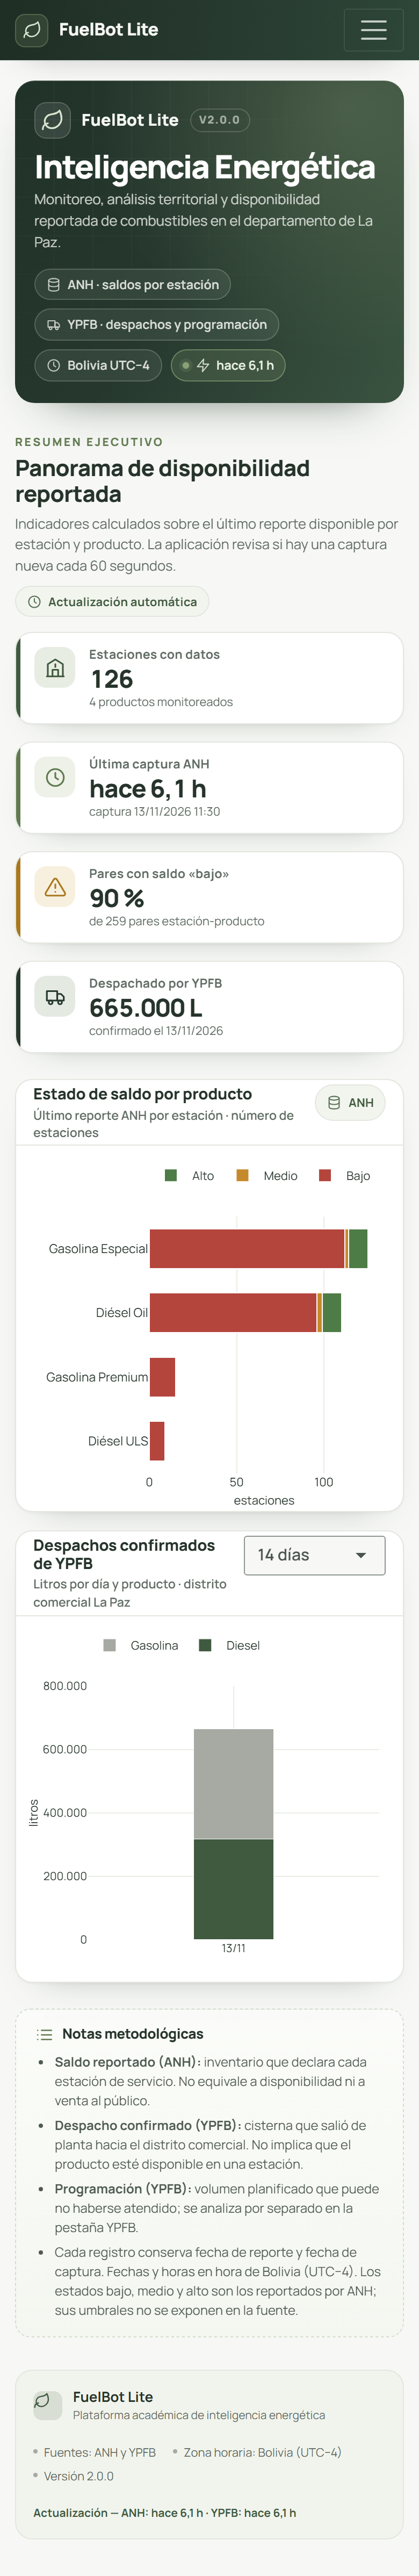
\includegraphics[width=\linewidth,height=0.54\textheight,keepaspectratio]{resumen_movil.png}
\caption{Resumen en 390 px.}
\end{subfigure}
\hfill
\begin{subfigure}{0.62\linewidth}
\centering

\includegraphics[width=\linewidth,height=0.54\textheight,keepaspectratio]{resumen.png}
\caption{Resumen en escritorio.}
\end{subfigure}
\caption{Comparación de la vista Resumen en móvil y escritorio.}
\label{fig:responsive}
\end{figure}

\subsection{Evaluación interna del rediseño}

\begin{table}[H]
\centering
\small
\caption{Evaluación interna del rediseño visual y funcional.}
\label{tab:score}
\begin{tabular}{@{}lrr@{}}
\toprule
\textbf{Criterio} & \textbf{Peso} & \textbf{Puntaje} \\
\midrule
Calidad visual y UI/UX & 25 & 24,0 \\
Conservación funcional & 25 & 24,0 \\
Calidad de visualizaciones & 15 & 13,5 \\
Interactividad & 10 & 9,5 \\
Responsividad & 10 & 9,5 \\
Arquitectura y mantenibilidad & 10 & 9,0 \\
Documentación & 5 & 5,0 \\
\midrule
\textbf{Total} & \textbf{100} & \textbf{94,5} \\
\bottomrule
\end{tabular}
\end{table}

El puntaje es una evaluación interna, no una calificación externa. Se apoya en las pruebas de la Tabla \ref{tab:pruebas} y en las capturas. Las deducciones corresponden a la cobertura de un solo día, la densidad del mapa, las columnas ocultas en móvil y la ausencia de un despliegue cloud de la aplicación.

% ============================================================
% 11. DISCUSIÓN
% ============================================================
\section{Discusión}\label{sec:discusion}

\subsection{Aportes}

El principal aporte es la integración reproducible de fuentes públicas con semánticas distintas. La separación entre saldo reportado, despacho confirmado y programación evita conclusiones incorrectas. La trazabilidad combina cuatro elementos: copia cruda, hash, bitacora de ingesta y fechas de captura y reporte. La seguridad se diseño en profundidad: guardia SQL, rol de solo lectura, permisos sobre vistas y límites de filas y pasos.

En el plano académico, el proyecto demuestra un ciclo completo de ingeniería de datos: extracción, limpieza, modelado, carga idempotente, consulta, visualización y agentes. También documenta decisiones y límites, lo que permite evaluar el trabajo sin depender de una demostración en vivo.

\subsection{Limitaciones}

\begin{enumerate}[leftmargin=1.2cm]
  \item \textbf{Cobertura temporal:} la instancia consultada contiene datos de un solo día. El pipeline admite backfill, pero no se cargó el histórico completo en esta instancia.
  \item \textbf{Fragilidad del scraping:} un cambio en el HTML de YPFB o en el JSON de ANH puede romper el extractor. El pipeline lo registra como error y no inventa datos.
  \item \textbf{Despliegue de la app:} la aplicación se validó localmente; no hay manifiesto de despliegue cloud.
  \item \textbf{Mapa:} los marcadores se superponen en el área metropolitana y no hay clustering.
  \item \textbf{Móvil:} se ocultan columnas secundarias sin una fila expandible.
  \item \textbf{Agente:} la latencia es variable; una ejecución superó 60 segundos. La cuota no se sometió a prueba de estrés.
  \item \textbf{Dependencias externas:} Supabase, Gemini, Google Fonts y OpenStreetMap requieren internet.
  \item \textbf{Secreto preexistente:} el SQL del rol contiene una contraseña versionada; debe rotarse.
  \item \textbf{Actualización automática:} el latido de 60 segundos esta implementado, pero no se observó una captura nueva durante la validación.
\end{enumerate}

\subsection{Validez y reproducibilidad}

La validez descriptiva se apoya en consultas directas a las vistas y en capturas de la interfaz. No se realizo una validación contra una fuente independiente de verdad, por lo que los resultados deben interpretarse como lo reportado por ANH y YPFB, no como una medición física de disponibilidad. La reproducibilidad depende de conservar las versiones de R y paquetes, los scripts SQL, las credenciales y el acceso a las fuentes. El repositorio documenta los pasos, pero la base y las claves son externas.

% ============================================================
% 12. CONCLUSIONES
% ============================================================
\section{Conclusiones y trabajo futuro}

\subsection{Conclusiones}

FuelBot Lite logra un flujo completo y trazable desde portales públicos hasta un tablero y un agente conversacional. La base en Supabase cumple el papel de capa persistente y de contrato de consulta; las vistas separan la semántica de los datos operativos. El rol de solo lectura y la guardia SQL reducen la superficie de riesgo del agente. La aplicación demuestra que es posible ofrecer análisis interactivo con datos reales, sin inventar cifras y declarando las limitaciones.

La validación confirma el arranque, la navegación, los filtros, el mapa, las tablas y el agente. También confirma que el rol de lectura no puede acceder a las tablas. El trabajo no demuestra un despliegue cloud de la aplicación ni una carga histórica completa; esas son tareas pendientes, no resultados ocultos.

\subsection{Trabajo futuro}

\begin{enumerate}[leftmargin=1.2cm]
  \item Cargar y validar el histórico completo del repositorio de referencia.
  \item Publicar la aplicación en un servicio cloud con secretos, HTTPS y límites de tiempo.
  \item Agregar clustering o agregación espacial al mapa.
  \item Incorporar una fila expandible para las columnas ocultas en móvil.
  \item Automatizar pruebas de regresión del pipeline y del agente.
  \item Rotar la contraseña del rol y eliminar el secreto del historial.
  \item Explorar agregados materializados para las consultas más frecuentes.
  \item Documentar un tablero de calidad de datos con capturas faltantes y cambios de estructura.
\end{enumerate}

% ============================================================
% REFERENCIAS
% ============================================================
\newpage
\addcontentsline{toc}{section}{Referencias}
\begin{thebibliography}{99}

\bibitem{r}
R Core Team.
\emph{R: A Language and Environment for Statistical Computing}.
Versión 4.6.2.
\url{https://www.r-project.org/}

\bibitem{shiny}
Posit.
\emph{Shiny: web application framework for R}.
\url{https://shiny.posit.co/}

\bibitem{bslib}
Posit.
\emph{bslib: Custom Bootstrap themes for Shiny}.
\url{https://rstudio.github.io/bslib/}

\bibitem{leaflet}
Cheng, J., Karambelkar, B. y Xie, Y.
\emph{Leaflet for R}.
\url{https://rstudio.github.io/leaflet/}

\bibitem{plotly}
Plotly Technologies Inc.
\emph{Plotly R Open Source Graphing Library}.
\url{https://plotly.com/r/}

\bibitem{dt}
Xie, Y., Cheng, J. y Tan, X.
\emph{DT: A Wrapper of the JavaScript Library DataTables}.
\url{https://rstudio.github.io/DT/}

\bibitem{supabase}
Supabase.
\emph{Supabase Documentation}.
\url{https://supabase.com/docs}

\bibitem{postgres}
PostgreSQL Global Development Group.
\emph{PostgreSQL Documentation}.
\url{https://www.postgresql.org/docs/}

\bibitem{gemini}
Google.
\emph{Gemini API: Function calling}.
\url{https://ai.google.dev/gemini-api/docs/function-calling}

\bibitem{actions}
GitHub.
\emph{GitHub Actions Documentation}.
\url{https://docs.github.com/actions}

\bibitem{osm}
OpenStreetMap contributors.
\emph{OpenStreetMap}.
\url{https://www.openstreetmap.org/}

\bibitem{anh}
Agencia Nacional de Hidrocarburos.
\emph{Portal de abastecimiento de combustibles}.
\url{https://abastecimiento.prod.anh.gob.bo}

\bibitem{ypfb}
Yacimientos Petrolíferos Fiscales Bolivianos.
\emph{Consulta de despachos y programación}.
\url{https://consulta.ypfb.gob.bo/}

\bibitem{repo}
Sociedad de Datos.
\emph{bo-combustible: datos abiertos de combustibles en Bolivia}.
\url{https://github.com/sociedatos/bo-combustible}

\end{thebibliography}

% ============================================================
% APÉNDICES
% ============================================================
\newpage
\appendix
\section{Inventario de scripts}

\begin{longtable}{@{}>{\raggedright\arraybackslash}p{0.38\linewidth}>{\raggedright\arraybackslash}p{0.55\linewidth}@{}}
\caption{Archivos principales del proyecto.}\\
\toprule
\textbf{Archivo} & \textbf{Función} \\
\midrule
\endfirsthead
\toprule
\textbf{Archivo} & \textbf{Función} \\
\midrule
\endhead
\path{pipeline/run_pipeline.R} & Orquestador de modos anh, ypfb, todo, backfill y backfill-local. \\
\path{pipeline/00_config.R} & Configuración, HTTP, crudos, normalización de fechas y conexiones. \\
\path{pipeline/01_extraer_anh.R} & Extracción y normalización de ANH. \\
\path{pipeline/02_extraer_ypfb.R} & Extracción del bloque JSON de YPFB. \\
\path{pipeline/03_backfill_repo.R} & Descarga de CSV históricos y backfill. \\
\path{pipeline/04_cargar_supabase.R} & Carga idempotente y bitacora. \\
\path{sql/01_esquema.sql} & Esquema \fuel{}, tablas e índices. \\
\path{sql/02_vistas_y_rol.sql} & Vistas, rol de lectura y permisos. \\
\path{agente/agente_gemini.R} & Function calling, guardia SQL y ejecución. \\
\path{agente/instrucciones.txt} & Reglas del agente y formato de respuesta. \\
\path{app.R} & Aplicación Shiny y orquestación. \\
\path{R/} & Modulos, tema, componentes y acceso a datos. \\
\path{www/motion.css} & Hoja de estilos activa. \\
\path{www/custom.js} & Interacciones del chat. \\
\path{.github/workflows/pipeline.yml} & Captura programada en GitHub Actions. \\
\bottomrule
\end{longtable}

\section{Comandos de ejecución}

\begin{lstlisting}[language=bash,caption={Secuencia de ejecucion reproducida.}]
# 1. Instalar paquetes (una vez)
Rscript install_packages.R

# 2. Crear el esquema y las vistas en Supabase (editor SQL)
#    Ejecutar sql/01_esquema.sql y luego sql/02_vistas_y_rol.sql

# 3. Cargar historicos (opcional)
Rscript pipeline/run_pipeline.R backfill

# 4. Captura en vivo
Rscript pipeline/run_pipeline.R anh
Rscript pipeline/run_pipeline.R ypfb

# 5. Ejecutar el tablero
Rscript -e 'shiny::runApp(".")'
\end{lstlisting}

\section{Glosario}

\begin{description}[leftmargin=1.2cm]
  \item[ETL] Extracción, transformación y carga de datos.
  \item[Idempotencia] Propiedad por la cual repetir una operación no duplica ni altera el resultado esperado.
  \item[Upsert] Inserción con actualización condicional ante conflicto.
  \item[Vista] Consulta almacenada que presenta una interfaz estable sobre las tablas.
  \item[Rol] Identidad de PostgreSQL con privilegios definidos.
  \item[Function calling] Mecanismo por el cual un modelo solicita la ejecución de una herramienta.
  \item[Crudo] Respuesta original de la fuente, conservada para auditoría.
  \item[Latido] Consulta periódica que detecta cambios en la base.
\end{description}

\section{Declaración de verificabilidad}

Las cifras de la sección \ref{sec:validacion} se obtuvieron de la instancia real del proyecto y de capturas generadas con Chrome headless. No se simularon respuestas de Supabase ni de Gemini. Las pruebas que no se ejecutaron se indican como tales: carga histórica completa, ejecución real del workflow en GitHub Actions, despliegue cloud de la aplicación y prueba de estrés de la cuota del agente.

\end{document}
